\documentclass{beamer}


% Beamer settings
\usecolortheme{rose}
\beamertemplatenavigationsymbolsempty
\setbeamertemplate{footline}[frame number]

\titlegraphic{%

\includegraphics[height=1cm]{logo-full-colour.png}}

\addtobeamertemplate{frametitle}{}{%
\begin{tikzpicture}[remember picture,overlay]
\node[anchor=north east,yshift=2pt] at (current page.north east) {
\includegraphics[height=1cm]{logo-full-colour.png}};
\end{tikzpicture}}

% Packages
\usepackage{amsmath}

\usepackage{tikz}
\usetikzlibrary{positioning}
\usetikzlibrary{fit}

\usepackage{pgfplots}
\usepgfplotslibrary{fillbetween}

\usepackage{minted}
\usepackage[T1]{fontenc} % Required by minted to ensure dollar signs are produced instead of pound (sterling) signs

\usepackage{multicol}

\usepackage{booktabs}

\usepackage{adjustbox}

% Author
\author{Simon McIntosh-Smith \& Tom Deakin\\University of Bristol}

\date{}



\title{OpenMP for Computational Scientists}
\subtitle{6: Tasking and Tools}

\begin{document}

\frame{\titlepage}

%-------------------------------------------------------------------------------
\begin{frame}
\frametitle{Outline}
\begin{itemize}
  \item Poor mans tasking: sections
  \item The single and master constructs
  \item Tasking in OpenMP
  \item Tools
\end{itemize}
\end{frame}

%-------------------------------------------------------------------------------
\begin{frame}[fragile]
\frametitle{The need for tasks}
\begin{itemize}
  \item What if your code doesn't follow a standard parallel loop pattern?
  \item OpenMP needs to know the loop count at runtime.
  \item Recursive and tree/graph based algorithms inconvenient to program with parallel loops.
  \item Tasking allows you to package work and data into units (tasks) and have them scheduled in parallel.
\end{itemize}

\begin{minted}[frame=single]{fortran}
p => head
do while(associated(p))
  call process(p)
  p => p%next
end do
\end{minted}
\end{frame}
%-------------------------------------------------------------------------------
\section{Sections}
\begin{frame}[fragile]
\frametitle{Sections}
\begin{itemize}
  \item Sections give you a way to assign different work to different threads.
  \item Useful for a producer/consumer pattern, but not really recursive algorithms.
  \item If fewer sections than threads, threads sit idle.
  \item If more sections than threads, sections assigned by implementation.
\end{itemize}

\begin{minted}[frame=single]{fortran}
!$omp parallel sections
    !$omp section
    call work1()

    !$omp section
    call work2()

!$omp end parallel sections
\end{minted}
\end{frame}

%-------------------------------------------------------------------------------
\section{Single and master}
\begin{frame}[fragile]
\frametitle{The single construct}
\begin{itemize}
  \item Often necessary for only one thread to do some work in a parallel region.
  \item Wrapping code with the \mintinline{fortran}|single| constructs means only one thread in the parallel region will execute that code.
  \item Not defined which thread will actually execute the block.
  \item There is an implicit barrier for this construct (can avoid with \mintinline{fortran}|nowait| clause).
\end{itemize}

\begin{minted}[frame=single]{fortran}
!$omp parallel
  call do_work()
  !$omp single
  call exchange_halos()
  !$omp end single
!$omp end parallel
\end{minted}
\end{frame}

%-------------------------------------------------------------------------------
\begin{frame}[fragile]
\frametitle{The master construct}
\begin{itemize}
  \item Similar to \mintinline{fortran}|single| construct, except guaranteed the master thread will execute the block.
  \item There is \emph{no} implicit barrier for this construct!
  \item Useful for cases where synchronisation isn't required:
    \begin{itemize}
      \item Printing out messages to the screen.
      \item Generating tasks!
    \end{itemize}
\end{itemize}

\begin{minted}[frame=single]{fortran}
!$omp parallel
  call do_work()
  if (conv .eq. .true.)
    !$omp master
    print *, "Converged!"
    !$omp end master
    exit
  end if
!$omp end parallel
\end{minted}
\end{frame}

%-------------------------------------------------------------------------------
\section{Tasks}
\begin{frame}[fragile]
\frametitle{Tasks}
\begin{itemize}
  \item OpenMP 3.0 introduced real tasking.
  \item Later versions refined and added features.
\end{itemize}

\begin{columns}
\begin{column}{0.5\textwidth}
\begin{minted}[frame=single,fontsize=\small]{fortran}
!$omp parallel
  !$omp master
    !$omp task
    call do_task(x,y,z)
    !$omp end task

    !$omp task
    call do_task(i,j,k)
    !$omp end task
  !$omp end master
!$omp end parallel
\end{minted}
\end{column}

\begin{column}{0.5\textwidth}
\begin{itemize}
  \item Use master thread to generate tasks for all threads to do.
  \item Idle threads take tasks off the task queue.
  \item Barrier at the \mintinline{fortran}|end parallel| ensures all tasks complete.
\end{itemize}
\end{column}
\end{columns}

\end{frame}

%-------------------------------------------------------------------------------
\begin{frame}
\frametitle{Trees}
Useful to think about tasks organised as a tree (or graph).

\begin{columns}
\begin{column}{0.5\textwidth}
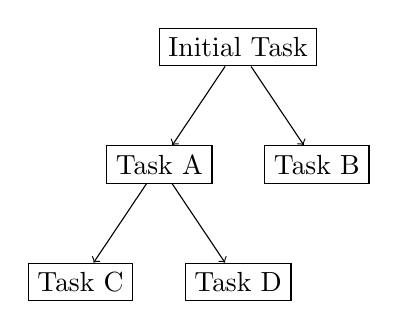
\begin{tikzpicture}[every node/.style = {shape=rectangle, draw}]
  \node (it) {Initial Task};
  \node (t1) [below=of it, xshift=-1cm] {Task A} edge [<-] (it);
  \node (t2) [below=of it, xshift=1cm] {Task B} edge [<-] (it);
  \node (t3) [below=of t1, xshift=-1cm] {Task C} edge [<-] (t1);
  \node (t4) [below=of t1, xshift=1cm] {Task D} edge [<-] (t1);

\end{tikzpicture}
\end{column}

\begin{column}{0.5\textwidth}
\begin{itemize}
  \item The Initial Task is the \emph{parent} of Task A.
  \item Task A is the \emph{child} of the Initial Task.
  \item Task A and Task B are \emph{siblings}.
\end{itemize}
\end{column}
\end{columns}
\end{frame}

%-------------------------------------------------------------------------------
\begin{frame}
\frametitle{Under the hood}
\begin{itemize}
  \item It's useful to think about how the OpenMP runtime itself implements tasking.
  \item In general, the runtime maintains a queue of tasks.
  \item Threads enqueue and dequeue tasks from the queue.
\end{itemize}

\begin{center}
\begin{adjustbox}{max width={\textwidth}}
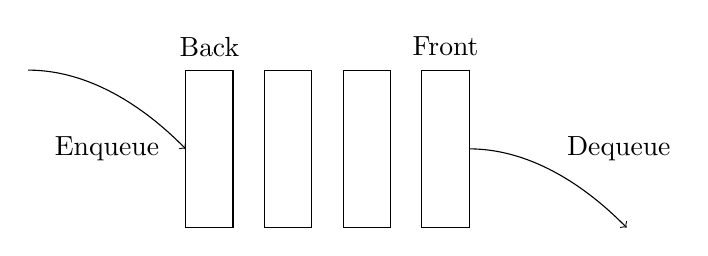
\begin{tikzpicture}
  \foreach \i in {0,...,3} {
    \draw (\i,0) rectangle (\i+.6,2);
  }
  \draw (3.3,2.3) node {Front};
  \draw (0.3,2.3) node {Back};

  \draw[->] (3.6,1) parabola (5.6,0);
  \draw (5.5,1) node {Dequeue};

  \draw[->] (-2,2) parabola (0,1);
  \draw (-1,1) node {Enqueue};
\end{tikzpicture}
\end{adjustbox}
\end{center}

\begin{itemize}
  \item Intel/Clang runtime has one task queue per thread, and allows work-stealing.
  \item Gives lower contention than case where all threads access a single queue.
\end{itemize}

\end{frame}

%-------------------------------------------------------------------------------
\subsection{Data sharing clauses}
\begin{frame}
\frametitle{Data sharing clauses}
\begin{itemize}
  \item Can use these three data sharing clauses from \mintinline{fortran}|parallel| regions on the \mintinline{fortran}|task| construct.
  \item The definitions are really the same, but applied to tasks, not threads.
  \item Need to think carefully about the appropriate clauses for each variable.
  \item \mintinline{fortran}|shared(x)|: There is one copy of the \mintinline{fortran}|x| variable, shared between the current and child tasks.
  \item \mintinline{fortran}|private(x)|: Each task gets its own local \mintinline{fortran}|x| variable. It is not initialised.
  \item \mintinline{fortran}|firstprivate(x)|: Each task gets its own local \mintinline{fortran}|x| variable. It is initialised to the value of the original variable in the encountering task region.
\end{itemize}
\end{frame}

%-------------------------------------------------------------------------------
\begin{frame}
\frametitle{Default data sharing}
\begin{itemize}
  \item Tasks and parallel regions have different default data sharing rules.
  \item By default, data is \emph{shared} for \mintinline{fortran}|parallel| regions.
  \item By default, data is \emph{firstprivate} for \mintinline{fortran}|task| constructs.
  \item Unless, it's shared by the enclosing (the outer) region.
  \item Using \mintinline{fortran}|default(none)| is recommended here especially.
\end{itemize}
\end{frame}

%-------------------------------------------------------------------------------
\subsection{Task synchronisation}
\begin{frame}
\frametitle{Task completion}
Three places where tasks synchronise:
\begin{enumerate}
  \item At thread barriers:
    \begin{itemize}
      \item Implicit barriers (like at end of \mintinline{fortran}|parallel| regions).
      \item Explicit \mintinline{fortran}|barrier| constructs.
    \end{itemize}
  \item At the \mintinline{fortran}|taskwait| construct:
    \begin{itemize}
      \item Waits on all child tasks of the current task before continuing.
      \item Only applies to tasks that the current task generated.
      \item Everything in OpenMP is defined as task, so here the ``outer'' task is the one that called the first \mintinline{fortran}|task| construct.
    \end{itemize}
  \item At the end of the \mintinline{fortran}|taskgroup| construct:
    \begin{itemize}
      \item Waits on all child tasks generated within the \mintinline{fortran}|taskgroup| region.
      \item Like \mintinline{fortran}|taskwait|, but allows grouping of child tasks.
    \end{itemize}
\end{enumerate}
\end{frame}

%-------------------------------------------------------------------------------
\begin{frame}
\frametitle{Taskwait: back to the tree}

\begin{columns}
\begin{column}{0.5\textwidth}
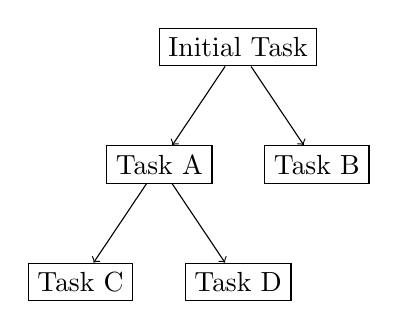
\begin{tikzpicture}[every node/.style = {shape=rectangle, draw}]
  \node (it) {Initial Task};
  \node (t1) [below=of it, xshift=-1cm] {Task A} edge [<-] (it);
  \node (t2) [below=of it, xshift=1cm] {Task B} edge [<-] (it);
  \node (t3) [below=of t1, xshift=-1cm] {Task C} edge [<-] (t1);
  \node (t4) [below=of t1, xshift=1cm] {Task D} edge [<-] (t1);
\end{tikzpicture}
\end{column}

\begin{column}{0.5\textwidth}
\begin{itemize}
  \item A \mintinline{fortran}|taskwait| in the Initial Task will wait for Task A and B to finish. Task A finishes when Tasks C and D are also finished.
  \item A \mintinline{fortran}|taskwait| in Task A will wait for Tasks C and D to finish.
  \item A \mintinline{fortran}|taskwait| in Task B will do nothing (no children).
\end{itemize}
\end{column}
\end{columns}
\end{frame}

%-------------------------------------------------------------------------------
\begin{frame}[fragile]
\frametitle{Taskgroup}
\begin{columns}
\begin{column}{.5\textwidth}
\begin{minted}[frame=single,linenos]{fortran}
!$omp parallel
!$omp master
  !$omp task
  call background_task()
  !$omp end task

  !$omp taskgroup
    !$omp task
    call recursive_task()
    !$omp end task
  !$omp end taskgroup

!$omp end master
!$omp end parallel
\end{minted}
\end{column}

\begin{column}{.5\textwidth}
\begin{itemize}
  \item Start a background task.
  \item The \mintinline{fortran}|recursive_task()| will generate many more tasks.
  \item All these tasks are children of the master task.
  \item A \mintinline{fortran}|taskwait| on line 11 would wait for \emph{all the tasks}, including the background task.
  \item The \mintinline{fortran}|taskgroup| waits for all the tasks in the group only, not including the background task.
\end{itemize}
\end{column}
\end{columns}

\end{frame}

%-------------------------------------------------------------------------------
\subsection{Fibonacci example}
\begin{frame}[fragile]
\frametitle{Fibonacci}
\begin{columns}
\begin{column}{0.5\textwidth}
\begin{minted}[breaklines,frame=single,linenos,fontsize=\small]{fortran}
recursive integer function fib(n) result(res)
  integer :: n, i, j
  if (n .lt. 2) then
    res = n
  else
    !$omp task shared(i)
    i = fib(n-1)
    !$omp end task
    !$omp task shared(j)
    j = fib(n-2)
    !$omp end task
    !$omp taskwait
    res = i+j
  end if
end function
\end{minted}
\end{column}

\begin{column}{0.5\textwidth}
\begin{itemize}
  \item Routine called from a parallel region by one of the threads.
  \item This first task \mintinline{fortran}|fib(40)| creates two tasks: \mintinline{fortran}|fib(39)| and \mintinline{fortran}|fib(38)|.
  \item \mintinline{fortran}|i| and \mintinline{fortran}|j| must be \mintinline{fortran}|shared| so that the results are retained by the calling task.
  \item The \mintinline{fortran}|taskwait| construct ensures that the child tasks are finished before summing their return values.
\end{itemize}
\end{column}

\end{columns}
NB: there are better ways to calculate Fibonacci numbers\dots
\end{frame}

%-------------------------------------------------------------------------------
\subsection{Dependencies}
\begin{frame}
\frametitle{Task dependencies}
\begin{itemize}
  \item OpenMP gives you the ability to define an ordering of tasks based on input and output data dependencies.
  \item In other words, can make tasks wait for other sibling tasks to finish before starting.
  \item Need to specify input and output dependencies.
  \item Only checks for previously generated siblings with a dependency specified.
  \item \mintinline{fortran}|depend(in: A)|: task depends on siblings with \mintinline{fortran}|out| or \mintinline{fortran}|inout| dependency \mintinline{fortran}|A|.
  \item \mintinline{fortran}|depend(out: A)|: task depends on siblings with any dependency on \mintinline{fortran}|A|.
  \item \mintinline{fortran}|depend(inout: A)|: same as \mintinline{fortran}|depend(out: A)|.
\end{itemize}
\end{frame}

%-------------------------------------------------------------------------------
\begin{frame}[fragile]
\frametitle{Dependency example}
\begin{columns}
\begin{column}{0.7\textwidth}
\begin{minted}[frame=single,linenos,fontsize=\small]{fortran}
!$omp task depend(out: x)
x = 1.0
!$omp end task

!$omp task depend(in: x) depend(out: y)
y = f(x)
!$omp end task

!$omp task depend(in: x) depend(out: z)
z = g(x)
!$omp end task

!$omp task depend(in: y, z)
print *, y+z
!$omp end task
\end{minted}
\end{column}

\begin{column}{0.3\textwidth}
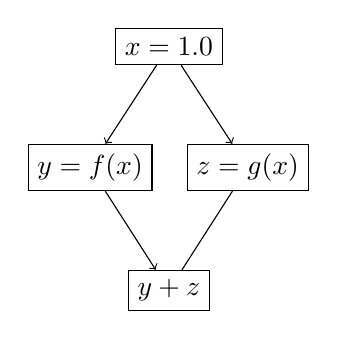
\begin{tikzpicture}[every node/.style = {shape=rectangle, draw}]
  \node (it) {$x = 1.0$};
  \node (t1) [below=of it, xshift=-1cm] {$y=f(x)$} edge [<-] (it);
  \node (t2) [below=of it, xshift=1cm] {$z=g(x)$} edge [<-] (it);
  \node (t3) [below=of t2, xshift=-1cm] {$y+z$} edge [<-] (t1) edge (t2);
\end{tikzpicture}
\end{column}
\end{columns}
\end{frame}

%-------------------------------------------------------------------------------
\begin{frame}[fragile]
\frametitle{Dependency example}
\begin{columns}
\begin{column}{0.5\textwidth}
\begin{minted}[breaklines,frame=single,linenos,fontsize=\small]{fortran}
!$omp task depend(out: x)
x = 1.0
!$omp end task

!$omp task depend(in: x) depend(out: y)
y = f(x)
!$omp end task

!$omp task depend(in: x) depend(out: z)
z = g(x)
!$omp end task

!$omp task depend(in: y, z)
print *, y+z
!$omp end task
\end{minted}
\end{column}

\begin{column}{0.5\textwidth}
\begin{itemize}
  \item Must specify first \mintinline{fortran}|out| dependency.
  \item Then generate $y=f(x)$ tasks which depends on it.
  \item Then generate $z=g(x)$ task, which depends on first but not second.
  \item Generate task which depends on middle two tasks.
  \item Note, OpenMP still sees all these tasks as \emph{siblings}.
\end{itemize}
\end{column}
\end{columns}

\end{frame}

%-------------------------------------------------------------------------------
\begin{frame}
\frametitle{New dependency clauses}
OpenMP 5.0 will introduce the \mintinline{fortran}|mutexinoutset| dependency qualifier.
\begin{itemize}
  \item Ensures commutativity between tasks depending on \mintinline{fortran}|x|.
  \item Sibling tasks with \mintinline{fortran}|depend(inout: x)| would need to be run in the order the tasks were generated.
  \item \mintinline{fortran}|mutexinoutset| means they can run in any order, not just the generated order.
  \item Tasks still won't run in parallel.
\end{itemize}
\end{frame}

%-------------------------------------------------------------------------------
\begin{frame}[fragile]
\frametitle{mutexinoutset}
\begin{columns}
\begin{column}{.5\textwidth}
\begin{minted}[breaklines,frame=single,fontsize=\small]{fortran}
!$omp task (inout: y)
call slow(y) ! Task A
!$omp end task

!$omp task (inout: z)
call fast(z) ! Task B
!$omp end task

!$omp task depend(inout: res) depend(in: y)
res = res + y ! Task C
!$omp end task

!$omp task depend(inout: res) depend(in: z)
res = res + z ! Task D
!$omp end task
\end{minted}
\end{column}

\begin{column}{.5\textwidth}
\begin{itemize}
  \item Task A and B will start.
  \item Task C can start once Task A has finished.
  \item Task D can start once both Tasks B and C have finished.
  \item Ideally should just wait on Task B, not C.
  \item Solved by replacing \mintinline{fortran}|depend(inout: res)| with \mintinline{fortran}|depend(mutexinoutset: res)|.
\end{itemize}
\end{column}
\end{columns}

\end{frame}

%-------------------------------------------------------------------------------
\subsection{Suspending tasks}
\begin{frame}
\frametitle{Suspending tasks with taskyield}
\begin{itemize}
  \item Once a task starts executing, it goes to completion unless it encounters a \emph{task scheduling point}.
  \item At these points, the threads can pick another task to start executing or resume a task.
  \item These points occur when you:
    \begin{itemize}
      \item Generate a task
      \item Finish a task
      \item Reach the end of a \mintinline{fortran}|taskgroup| construct.
      \item Synchronise with \mintinline{fortran}|barrier| or \mintinline{fortran}|taskwait|.
      \item And, at a \mintinline{fortran}|taskyield| construct.
    \end{itemize}
   \item The \mintinline{fortran}|taskyield| construct allows tasks to be suspended so another task can start.
   \item Really useful when polling for a lock, otherwise the task never ``sleeps''.
   \item Not all implementations actually suspend tasks (Intel/Clang does).
\end{itemize}
\end{frame}

%-------------------------------------------------------------------------------
\begin{frame}[fragile]
\frametitle{taskyield example}
\begin{minted}[linenos,frame=single,breaklines]{fortran}
!$omp task
  call do_something()

  ! Wait for the lock
  do while (.not. omp_test_lock(lock))
    ! Couldn't get lock, so suspend task and schedule another
    !$omp taskyield
  end do

  ! Only one task should call this function
  call critical_code()

  ! Release the lock
  call omp_unset_lock(lock)
!$omp end task
\end{minted}

\end{frame}

%-------------------------------------------------------------------------------
\subsection{Generating lots of tasks}
\begin{frame}[fragile]
\frametitle{The taskloop construct}

\begin{itemize}
  \item Generates a task for each loop iteration.
  \item Shorthand for generating tasks in a tiled \mintinline{fortran}|parallel do| loop.
  \item Tasks form part of a \mintinline{fortran}|taskgroup|, unless use the \mintinline{fortran}|nogroup| clause.
  \item \mintinline{fortran}|grainsize(num)| clause: sets the minimum number of iterations for each generated task.
  \item \mintinline{fortran}|num_tasks(num)| clause: set number of tasks to create. Unlikely to want to specify this in practice.
  \item \mintinline{fortran}|collapse| clause can also be used.
\end{itemize}

\begin{minted}[frame=single]{fortran}
!$omp taskloop
do i = 1, N
  call do_work(i)
end do
!$omp end taskloop
\end{minted}

\end{frame}
%-------------------------------------------------------------------------------
\subsection{Summary}
\begin{frame}
\frametitle{Other clauses}
Some rare clauses you can use when generating tasks, but unlikely to use them in most cases.
\begin{itemize}
  \item \mintinline{fortran}|untied|: If the task gets suspended, any thread can start it. Without this clause, the thread which started the task must resume it. Helpful for load balancing when used with \mintinline{fortran}|taskyield|.
  \item \mintinline{fortran}|mergeable|: The task can be merged into the parent task, sharing its data environment. Execution might happen straight away, or be delayed.
  \item \mintinline{fortran}|priority(n)|: The task is given a priority value $n \ge 0$. Gives a hint to the runtime about which tasks to run first.
  \item \mintinline{fortran}|final(expr)|: If the expression is true, this and all further child tasks are included in the parent task, and just executed immediately. Useful for specifying a minimum tasks size in recursive algorithms.
\end{itemize}
\end{frame}
%-------------------------------------------------------------------------------
\begin{frame}
\frametitle{Tasking advice}
\begin{itemize}
  \item Getting the correct data sharing clauses can be tricky.
  \item Don't use tasks for patterns supported by other parts of OpenMP (parallel loops).
  \item Tasking comes with overheads.
  \item The runtime is good, but can't work miracles.
  \item Best results obtained where use controls number and granularity of tasks.
\end{itemize}
\end{frame}

%-------------------------------------------------------------------------------
\section{Tools}
\begin{frame}
\frametitle{Tools}
Intel Parallel Studio XE
\begin{itemize}
  \item Intel Advisor
    \begin{itemize}
      \item Shows vectorisation efficiency and Roofline analysis.
      \item Can show you where might be good to thread, but obviously can't refactor your code for you to make it parallelisable.
    \end{itemize}

  \item Intel Inspector
    \begin{itemize}
      \item Debugger for memory errors and thread errors (such as deadlock).
    \end{itemize}

  \item Intel vTune Amplifier
    \begin{itemize}
      \item Performance tuning using hardware counters and metrics.
      \item Very detailed information presented, but tries to summarise it.
    \end{itemize}

  \item The documentation on the Intel website is really helpful.
\end{itemize}
\end{frame}

%-------------------------------------------------------------------------------
\begin{frame}
\frametitle{Tools}
ARM HPC Tools
\begin{itemize}
  \item From ARM, but cross-platform. Used to be the Allinea Forge tools.
  \item DDT: Graphical debugger. Really good for parallel programs in MPI and OpenMP (and both).
  \item Map: Simple to use profiler. Can show thread activity, synchronisation and communication overheads.
  \item \url{https://www.arm.com/products/development-tools/hpc-tools/cross-platform/forge}
\end{itemize}
\end{frame}

%-------------------------------------------------------------------------------
\begin{frame}
\frametitle{Tools}
Cray PerfTools
\begin{itemize}
  \item CrayPat
    \begin{itemize}
      \item Performance analysis tool for Cray systems.
      \item Gives overview of expensive routines and communication and synchronisation costs.
      \item Also uses hardware counters for more details information.
    \end{itemize}
  \item Reveal
    \begin{itemize}
      \item Analyses loop dependencies and uses performance data to automatically try to insert OpenMP constructs.
      \item Doesn't do a complete job, still need to check the constructs are correct.
      \item Obviously can't refactor a loop to make is parallelisable.
      \item \url{http://www.nersc.gov/users/software/performance-and-debugging-tools/craypat/reveal/}
    \end{itemize}
\end{itemize}
\end{frame}

%-------------------------------------------------------------------------------
\begin{frame}
\frametitle{Tools}
\begin{itemize}
  \item Can use the NVIDIA debuggers and profilers for OpenMP \mintinline{fortran}|target| constructs.
  \item Extrae and Paraver profiler and visualiser from Barcelona Supercomputing Center: \url{https://tools.bsc.es}.
  \item Score-P and Vampir: good for generating timelines of multi-threaded/process code: \url{https://www.alcf.anl.gov/files/Vampir.pdf}
  \item TAU profiler and program tracer: \url{https://www.cs.uoregon.edu/research/tau/tau.ppt}
  \item TotalView debugger: \url{https://computing.llnl.gov/tutorials/totalview/}
\end{itemize}
\end{frame}
%-------------------------------------------------------------------------------
\section{Exercise}
\begin{frame}
\frametitle{Exercise}
TODO: LU factorisation
\end{frame}

%-------------------------------------------------------------------------------
\begin{frame}
\frametitle{Resources}
\begin{itemize}
  \item SC'16 Tutorial from Tim Mattson and Alice Koniges: \url{https://www.nersc.gov/assets/Uploads/SC16-Programming-Irregular-Applications-with-OpenMP.pdf}
  \item Patrick Atkinson and Simon McIntosh-Smith, \emph{On the Performance of Parallel Tasking Runtimes for an Irregular Fast Multipole Method Application}, IWOMP 2017. \url{https://link.springer.com/chapter/10.1007/978-3-319-65578-9_7}.
\end{itemize}
\end{frame}
%-------------------------------------------------------------------------------

\end{document}

